\documentclass{beamer}
\usepackage[utf8]{inputenc}
\usepackage{capt-of}
\usepackage[american]{babel}
\usepackage{csquotes}
\usepackage[style=apa,backend=biber]{biblatex}
\usepackage{tikz}
\usepackage{mathrsfs}

\usetheme{Madrid}
\usecolortheme{default}

\let\oldfootnoterule\footnoterule
\def\footnoterule{\only<2->\oldfootnoterule}

\DeclareLanguageMapping{american}{american-apa}
\addbibresource{biblio.bib}
\setbeamertemplate{bibliography item}{\insertbiblabel}

%------------------------------------------------------------
%This block of code defines the information to appear in the
%Title page
\title[Defining Random Variables] %optional
{Defining Random Variables}

% \subtitle{}

\author[R. Mok] % (optional)
{R.~Mok BSc(AdvMath), MTeach, GradCertDS}

\date[November 2021] % (optional)
{AISNSW Focus Day, November 2021}

%End of title page configuration block
%------------------------------------------------------------



%------------------------------------------------------------
%The next block of commands puts the table of contents at the
%beginning of each section and highlights the current section:

\AtBeginSection[]
{
  \begin{frame}
    \frametitle{Table of Contents}
    \tableofcontents[currentsection]
  \end{frame}
}
%------------------------------------------------------------


\begin{document}

%The next statement creates the title page.
\frame{\titlepage}


%---------------------------------------------------------
%This block of code is for the table of contents after
%the title page
\begin{frame}
\frametitle{Table of Contents}
\tableofcontents
\end{frame}
%---------------------------------------------------------

\section{Purpose of Presentation}

%---------------------------------------------------------

\begin{frame}
\frametitle{Purpose of Presentation}
\begin{block}{The Problem}
\begin{itemize}
  \item<2-> The Syllabus attempts to define a random variable in terms of what it tries to achieve/model but doesn't actually define what it is:
    \begin{itemize}
      \item Define and categorise random variables
        \begin{itemize}
          \item know that a random variable describes some aspect in a population from which samples can be drawn
          \item know the difference between a discrete random variable and a continuous random variable
        \end{itemize}
    \end{itemize}
    \parencite[p.~47]{syllabus}
  \item<3-> The Syllabus glossary isn't a great definition at all:
    \begin{itemize}
      \item A random variable is a variable whose possible values are outcomes of a statistical experiment or random phenomenon.
        \parencite[p.~73]{syllabus}
    \end{itemize}
  \item<4-> The Cambridge Textbook just gives an \emph{example} of a random variable that models tossing 4 coins.
  \item<5-> It seems like no one really knows what a Random Variable is.
\end{itemize}
\end{block}
\end{frame}

\begin{frame}
\frametitle{Purpose of Presentation}
\begin{block}{Purpose}
  \begin{itemize}
    \item<2-> Define probability concepts properly such as Random Variables.
    \item<3-> This presentation will not concentrate on methods of computation with Random Variables.
    \item<4-> Why? Analogous to being able to \emph{compute} derivatives vs. \emph{understanding} derivatives, a deeper understanding of Random Variables enhances one's appreciation for the computations and applications.
    \item<5-> As a result, some of the material in this presentation is not in the Syllabus, or expands/corrects some concepts in the Syllabus.
  \end{itemize}
\end{block}
\end{frame}

\begin{frame}
\frametitle{Purpose of Presentation}
\begin{block}{\parencite[pp.~2-3]{analysis_tao}}
  There is a certain philosophical satisfaction in knowing \emph{why} things work... you can certainly use things like the chain rule, L'H\^{o}pital's rule, or integration by parts without knowing why these rules work, or whether there are exceptions to these rules. However, one can get into trouble if one applies rules without knowing where they came from and what the limits of their applicability are.
  % Page 2-3 Analysis I
\end{block}
\end{frame}

%---------------------------------------------------------

\section{Set and Function Preliminaries}

%---------------------------------------------------------

\begin{frame}
  \frametitle{Preliminaries}
  \begin{block}{Sets}
    A set is a collection of distinct objects. e.g. $A = \{1,2,a,\mbox{Dave}\}$, or $B = \{c, 2, \pi, \mathbb{H}, \mathfrak{g}\}$.
  \end{block}
  Recall the set operations:
  \begin{itemize}
    \item Union: $A \cup B = \{1,2,a,c,\pi,\mathbb{H},\mathfrak{g},\mbox{Dave}\}$
    \item Intersection: $A \cap B = \{2\}$
  \end{itemize}
  Recall that a set $C$ is a subset of $A$ if all elements of $C$ are also in $A$, and we write: $C \subseteq A$. Example: $\{1,\mbox{Dave}\}\subseteq A$.
\end{frame}
\begin{frame}
  \frametitle{Preliminaries}
  \begin{block}{Function}
    A function $f$ from a set $A$ into $B$, denoted $f: A \rightarrow B$ assigns to each $a \in A$ an element $f(a) = b \in B$.

    The set $A$ is called the \emph{domain} and the set $B$ is called the \emph{co-domain}.

    The \emph{range} is the set $\{ f(a) | a \in A \}$.
  \end{block}
  \begin{example}
    \begin{center}
    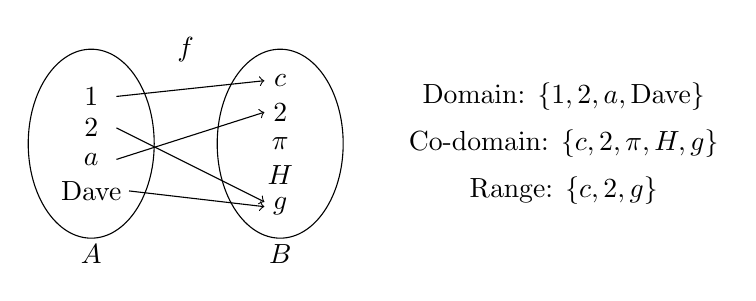
\begin{tikzpicture}[scale = .4]
      \draw (-3,-3.5) node {$A$} (3,-3.5) node {$B$};
      \draw (0,3) node {$f$};
      \draw (-3,0) ellipse (2 and 3);
      \draw (-3,1.5) node {$1$} (-3,0.5) node {$2$} (-3, -0.5) node {$a$} (-3,-1.5) node {Dave};
      \draw (3,2) node {$c$} (3,1) node {$2$} (3, 0) node {$\pi$} (3,-1) node {$\mathbb{H}$} (3,-2) node {$\mathfrak{g}$};
      \draw (3,0) ellipse (2 and 3);
      \draw[->] (-2.2,1.5) -- (2.5,2);
      \draw[->] (-2.2,0.5) -- (2.5,-1.85);
      \draw[->] (-2.2,-0.5) -- (2.5,1);
      \draw[->] (-1.8,-1.5) -- (2.5,-2);
      \pause
      \draw (12, 1.5) node {Domain: $\{1,2,a,\mbox{Dave}\}$};
      \draw (12, 0) node {Co-domain: $\{c,2,\pi,\mathbb{H},\mathfrak{g}\}$};
      \draw (12, -1.5) node {Range: $\{c, 2, \mathfrak{g}\}$};
    \end{tikzpicture}
  \end{center}
  \end{example}
\end{frame}

\begin{frame}
  \frametitle{Preliminaries}
  \begin{block}{Countable and Uncountable Sets}
    Two types of size (or cardinality) of sets that one encounters in mathematics are:
    \begin{itemize}
      \item Countable: elements in a countable set can be listed (enumerated), e.g the set of integers $\mathbb{Z}$, the set of rational numbers $\mathbb{Q}$, any finite set.
      \item Uncountable: elements in an uncountable set cannot be listed (enumerated). e.g. the set of real numbers $\mathbb{R}$, the real interval $[0,1]$.
    \end{itemize}
    \begin{center}
      $n(\mathbb{Z}) = n(\mathbb{Q}) < n(\mathbb{R})$
    \end{center}

  \end{block}
\end{frame}

% --------------------------------------------------------

\section{Probability Concepts as Sets}

% --------------------------------------------------------

\begin{frame}
  \frametitle{Sample Space}
  \begin{block}{Sample Space \parencite[p.~192]{measure_tao}}
    The Sample Space is the set of all possible states that a random system could be in, denoted $\Omega$.
  \end{block}
  \begin{example}
    Consider the coloured spinner:
    \begin{center}
    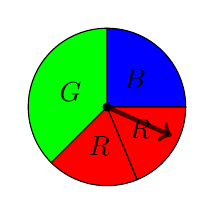
\begin{tikzpicture}
      \draw[fill=blue] (0,0) -- (1,0) arc (0:90:1) -- cycle;
      \draw[fill=red] (0,0) -- (1,0) arc (0:{-135/2}:1) -- cycle;
      \draw[fill=red] (0,0) -- ({cos(-135/2)},{sin(-135/2)}) arc ({-135/2}: -135: 1) -- cycle;
      \draw[fill=green] (0,0) -- (0,1) arc (90:225:1) -- cycle;
      \draw[ultra thick, ->, black, opacity = 0.7] (0,0) -- ({0.9*cos(-24)}, {0.9*sin(-24)});
      \draw[fill=black] (0,0) circle (0.05);
      \draw ({0.5*cos(45)}, {0.5*sin(45)}) node {$B$};
      \draw ({0.5*cos(-135/4)}, {0.5*sin(-135/4)}) node {$R$};
      \draw ({0.5*cos(-135/4*3)}, {0.5*sin(-135/4*3)}) node {$R$};
      \draw ({0.5*cos((90+225)/2)}, {0.5*sin((90+225)/2)}) node {$G$};
    \end{tikzpicture}
    \end{center}
    What is the sample space?
    \pause
    $\Omega = \{B, G, R\}$

    \pause
    It could also be: $\Omega = [0, 2\pi)$
  \end{example}
\end{frame}

\begin{frame}
  \frametitle{Events and Event Spaces}
  \begin{block}{Event \parencite[p.~192]{measure_tao}}
    An Event is a subset of the Sample Space.
  \end{block}
  \begin{example}
  The set $E = \{2,4,6\}$ would represent the Event of rolling even numbers on a 6-sided die with sample space $\Omega = \{1,2,3,4,5,6\}$.
  \end{example}
\end{frame}
\begin{frame}
  \begin{block}{Event Space \parencite[p.~192]{measure_tao}}
    An Event Space (also known as a sigma-field), $\mathscr{F}$, is the set of all possible Events that one can measure the probability of.
  \end{block}
  \begin{example}
    Continuing with the running example of the spinner on the previous slide, the Event Space would be:

    \begin{itemize}
      \item<2-> $\mathscr{F} = \{\{\}, \{B\}, \{G\}, \{R\}, \{B,G\}, \{B,R\}, \{G, R\}, \{B, G, R\}\}$
      \item<3-> What would $\mathscr{F}$ be if the Sample Space was $[0,2\pi)$? (Not in the scope of today's presentation - open for questions at the end of the presentation)
    \end{itemize}
  \end{example}
\end{frame}
\begin{frame}
  \frametitle{Probability Measure}
  \begin{block}{Probability Measure \parencite[p.~10]{daners}}
    The probability of an Event $E$, denoted $P(E)$, is a function $P: \mathscr{F} \rightarrow [0,1]$, and:
    \begin{itemize}
      \item For all $n \in \mathbb{N}$, if the events $E_1, E_2, \ldots, E_n \in \mathscr{F}$ are disjoint (i.e. they all have empty intersection), then $P(E_1 \cup E_2 \cup \ldots \cup E_n) = P(E_1) + P(E_2) + \ldots + P(E_n)$.
      \item $P(\{\}) = 0$
      \item $P(\Omega) = 1$
    \end{itemize}
  \end{block}
  \begin{example}
    \pause
    Continuing with the running example of the spinner with sample space $\Omega = \{B, G, R\}$, we can measure the probability of the Events with the following function:

    $P(\{\}) = 0$, $P(\{B\}) = \frac{1}{4}$, $P(\{G\}) = \frac{3}{8}$, $P(\{R\}) = \frac{3}{8}$. The probability of the other events can be found using the first property listed above.
  \end{example}
\end{frame}

\begin{frame}
  \frametitle{Summary So Far}
  \begin{block}{Summary So Far}
    \begin{itemize}
      \item<1-> Sets
      \item<2-> Functions $f: A \rightarrow B$, domain, co-domain, range
      \item<3-> Countable and Uncountable sets
      \item<4-> Sample Space $\Omega$
      \item<5-> Event Space $\mathscr{F}$
      \item<6-> Probability Measure $P: \mathscr{F} \rightarrow [0,1]$
      \item<6-> Note: A lot of references will call the triple $(\Omega, \mathscr{F}, P)$ a Probability Space.
    \end{itemize}
  \end{block}
\end{frame}

% --------------------------------------------------------

\section{Random Variables}

% --------------------------------------------------------

\begin{frame}
  \frametitle{Random Variables}
  \begin{alertblock}{Random Variable \parencite[p.~143]{daners}}
    A random variable $X$ is a \emph{function} $X: \Omega \rightarrow \mathbb{R}$.
    \begin{itemize}
      \item<2-> $X$ is a \emph{discrete random variable} if and only if the \emph{range} of $X$ is countable.
      \item<3-> $X$ is a \emph{continuous random variable} if and only if the \emph{range} of $X$ is uncountable.
    \end{itemize}
  \end{alertblock}
  \pause\pause\pause
  \begin{block}{Useful Notation for Random Variables}
    Some conventional notation:
    \begin{itemize}
      \item<5-> $[X = a] = \{\omega \in \Omega | X(\omega) = a\}$
      \item<6-> $[X < a] = \{\omega \in \Omega | X(\omega) < a\}$
      \item<7-> $[X > a] = \{\omega \in \Omega | X(\omega) > a\}$
      \item<8-> $[a < X < b] = \{\omega \in \Omega | a < X(\omega) < b\}$, etc
    \end{itemize}
  \end{block}
\end{frame}

\begin{frame}
  \frametitle{Example of Discrete Random Variable}
  \begin{example}
    \begin{center}
    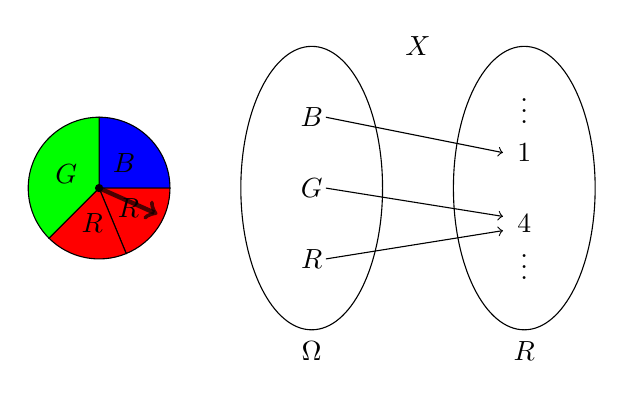
\begin{tikzpicture}[scale = 0.9]
      % draw the spinner
      \draw[fill=blue] (0,0) -- (1,0) arc (0:90:1) -- cycle;
      \draw[fill=red] (0,0) -- (1,0) arc (0:{-135/2}:1) -- cycle;
      \draw[fill=red] (0,0) -- ({cos(-135/2)},{sin(-135/2)}) arc ({-135/2}: -135: 1) -- cycle;
      \draw[fill=green] (0,0) -- (0,1) arc (90:225:1) -- cycle;
      \draw[ultra thick, ->, black, opacity = 0.7] (0,0) -- ({0.9*cos(-24)}, {0.9*sin(-24)});
      \draw[fill=black] (0,0) circle (0.05);
      \draw ({0.5*cos(45)}, {0.5*sin(45)}) node {$B$};
      \draw ({0.5*cos(-135/4)}, {0.5*sin(-135/4)}) node {$R$};
      \draw ({0.5*cos(-135/4*3)}, {0.5*sin(-135/4*3)}) node {$R$};
      \draw ({0.5*cos((90+225)/2)}, {0.5*sin((90+225)/2)}) node {$G$};

      % draw the random variable as internal diagrams
      \draw (4.5, 2) node {$X$};
      \draw (3,-2.3) node {$\Omega$};
      \draw (6,-2.3) node {$\mathbb{R}$};
      \draw (3,0) ellipse (1 and 2);
      \draw (6,0) ellipse (1 and 2);
      \pause
      \draw (3,1) node {$B$};
      \draw (3,0) node {$G$};
      \draw (3,-1) node {$R$};
      \pause
      \draw (6,1.2) node {$\vdots$};
      \draw (6,0.5) node {$1$};
      \draw (6,-0.5) node {$4$};
      \draw (6,-1) node {$\vdots$};

      \draw[->] (3.2, 1) -- (5.7, 0.5);
      \draw[->] (3.2, 0) -- (5.7, -0.4);
      \draw[->] (3.2, -1) -- (5.7, -0.6);
    \end{tikzpicture}
    \end{center}
  \end{example}
  \begin{itemize}
    \item<4-> Range: $\{1, 4\}$
    \item<5-> $[X = 4] = \{G, R\}$
    \item<6-> $[X > -1] = \{B, G, R\}$
    \item<7-> $[X > 100] = \{\}$
  \end{itemize}
\end{frame}

\begin{frame}
  \frametitle{Example of Continuous Random Variable}
  \begin{example}
    A machine with a slider moving between the values of $-2$ and $2$ inclusive prints a value equal to the square of where the slider lands.\\
    \pause
    $X: [-2, 2] \rightarrow \mathbb{R}$\\
    $X(\omega) = \omega^2$
  \end{example}
  \begin{itemize}
    \item<3-> Range: $[0,4]$
    \item<4-> $[X = 4] = \{2, -2\}$
    \item<5-> $[1 < X \leq 3] = [-\sqrt{3}, -1)\cup(1, \sqrt{3}]$
  \end{itemize}
\end{frame}

% --------------------------------------------------------

\section{Finding Probabilities of Random Variables}
% Finite sample space case -> just list out the probabilities of the singleton sets
% Infinite sample space case -> introduce concept of cumulative distribution function
% Mention nominally Radon-Nikodym Theorem that defines probability measure of the sample space via measure on the real numbers and derivative of the cumulative distribution function

% --------------------------------------------------------

\begin{frame}
  \frametitle{Easy Scenario: Finite Sample Spaces}
\end{frame}

% --------------------------------------------------------

\section{Application to Questions}

% --------------------------------------------------------

% --------------------------------------------------------

\section{Bibliography}

% --------------------------------------------------------

\begin{frame}
  \frametitle{Bibliography}
  \printbibliography

  Source files and PDF for this presentation can be found on:
  \url{https://github.com/moksifu/aisnsw_focus_day_2021}
  under the MIT Licence.
\end{frame}


%---------------------------------------------------------


\end{document}
